In the previous sections, we implicitly assumed that the raw movie of fluorescence measurements collected by the experimenter had undergone two stages of pre-processing.  First, the movie was segmented, to determine regions-of-interest (ROIs).  This yields a vector, $\vF_t$, corresponding to the fluorescence intensity at time $t$ for each of the $N_p$ pixels in the ROI.  Second, we projected that vector into a scalar, yielding $F_t$, the assumed input.  In this section, we still assume that somebody has gone through our movies and performed some segmentation, but we do not assume that they have projected the vector $\vF_t$ into a scalar $F_t$.  Formally, we posit a more general model:

\begin{align} \label{eq:bF}
\vF_t &= \valpha (C_t + \beta) +  \sig \vec{\varepsilon}_t, \qquad &\vec{\varepsilon}_t \sim \mathcal{N}(\vec{0},\bI)   
\end{align}

\noindent where $\vF_t$, $\valpha$, $\vec{\varepsilon}_t$, and $\vec{0}$  are all column vectors of length $N_p$, and $\bI$ is an $N_p \times N_p$ identity matrix.  This model follows from the observation that the fluorescence at any individual pixel is composed of a static element, $\beta$, and a dynamic element, that we assume is purely due to calcium fluctuations, $C_t$.  Further, we have assumed that the noise is uncorrelated and has the same variance, $\sig^2$, in each pixel (an assumption that can be relaxed quite easily).  Performing inference in this more general model proceeds nearly identical as before, 

\begin{align} 
\hbC_{\zzz} 
&= \az  \frac{1}{2 \sig^2} \norm{\vec{\bF} - \valpha (\bC\T +\beta\ve{1}\T)}^2 + (\bM \bC )\T \blam  - \zzz \log(\bM \bC)\T\ve{1},  \label{eq:eta4}\\
\ve{g} &= -\frac{\balpha}{\sig^2}(\bF -\balpha({\hbC\T}_{\zzz} + \beta)) + \ve{M}\T\blam - \zzz \ve{M}\T (\ve{M} \hbC_{\zzz})^{-1} \label{eq:g2} \\
\ve{H} &= \frac{\balpha\T \balpha}{\sig^2} \ve{I} + \zzz \ve{M}\T (\ve{M} \hbC_{\zzz})^{-2} \ve{M} \label{eq:H2}
\end{align}

Figure \ref{fig:spatial} demonstrates the utility of this generalization.  The top row shows different depictions of an ROI containing a single neuron, all using the same color scale.  On the far left panel is the ``true'' spatial filter.  Importantly, some pixels are \emph{anti-correlated} with others, as indicated by certain pixels being black, and others white.  Such a scenario can often arise in both in vitro and in vivo recordings, as the concentration of calcium immediately outside the cell often decreases after a spike, as the calcium ions flow into the cell.  Unsurprisingly, the mean frame looks very similar to the true spatial filter, as individual frames are effectively just modulating the magnitude of the spatial filter, and adding noise.  Typically, one would simply identify the pixels with high positive values from the mean frame, and average them together.  Such an approach yields the 1-dimensional fluorescence projection depicted on the left middle panel, with its associated inferred spike train beneath.  Using the true spatial filter to project $\vec{\bF}$ onto a 1-dimensional fluorescence time series results in the middle right panel, with its associated inferred spike train beneath.  It should be clear that using the true spatial filter improves the SNR of the fluorescence signal, and therefore, the inferred spike train accuracy.

\begin{figure}[H]
\centering 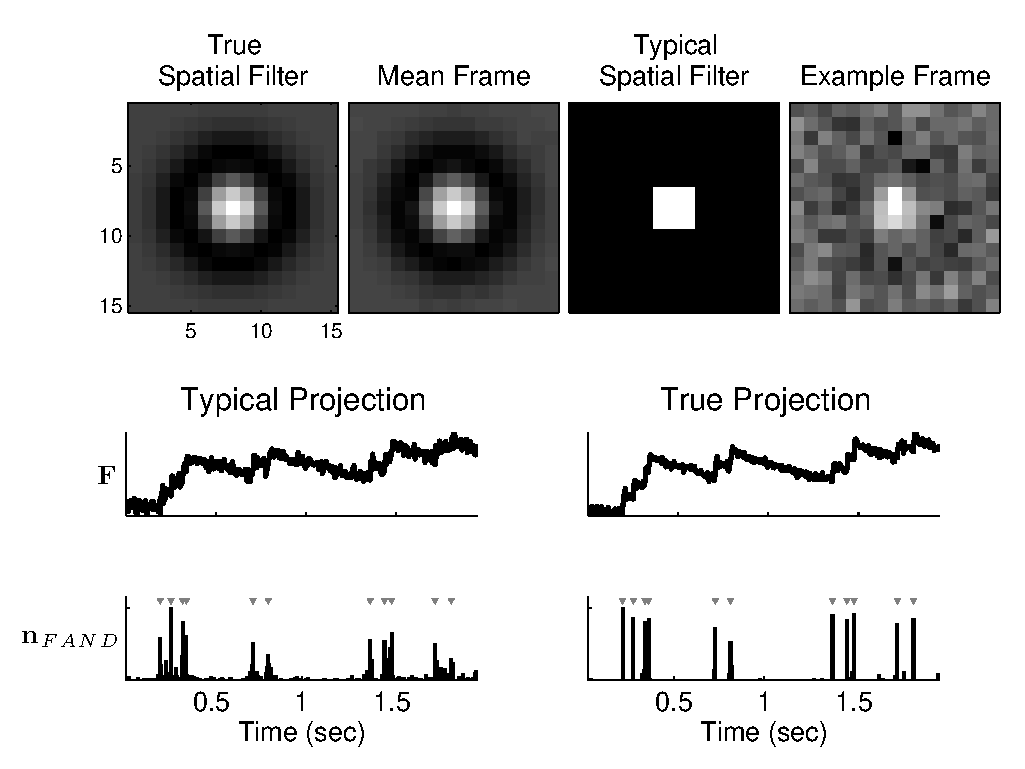
\includegraphics[width=.9\linewidth]{../figs/spatial}
\caption{A simulation demonstrating that using a better spatial filter can significantly enhance the effective SNR (see Supplementary Movie 1 for the full movie associated with this simulation).  Top: four movie frames.  Middle left: projection of the entire movie onto the optimal spatial filter, yielding a 1D fluorescence time series, with a large SNR. Bottom left: FAND filter's inferred spike train using the optimal spatial filter.  Middle right: projection of the entire movie onto the ``mean'' spatial filter, yielding a 1D fluorescence time series with a small SNR. Bottom right: FAND filter's inferred spike train using the mean spatial filter. Parameters different from Fig \ref{fig:schem}: $\balpha$ is a mixture of two 2D-Gaussians, with mean $\mu_1=\mu_2=[0, 0]$ and covariance matrices, $\Sigma_i=\sig_i^2 \ve{I}$, with $\sig_1=2$ and $\sig_2=4$ and $\ve{I}$ is the identity matrix. $\bbeta=1$.} \label{fig:spatial} \end{figure} 